\section{Aufbau}
\label{sec:Aufbau}

Die schematische Darstellung des Versuchsaufbaus ist in Abbildung \ref{fig:aufbau} zu sehen. An der Probe, ein Kupferblock mit einer Masse von \SI{342}{\gram},  ist eine Heizwicklung zur Erhitzung der Probe, sowie ein Pt-100 Messwiederstand zur Bestimmung der Temperatur angebracht.
Mit der Funktion
\begin{equation}
	T = 0,00134 R^2 + 2,296 R -243,02
	\label{eq:pt100}
\end{equation}
lässt sich aus den gemessenen Widerstand die Temperatur in °C bestimmen.
Die Probe befindet sich in einem Rezipienten, welcher ebenfalls geheizt werden, um den Wärmeaustausch der Probe mit der Umgebung möglichst gering zu halten. Dieser kann außerdem evakuiert oder mit Helium befüllt werden. Der Rezipient befindet sich in einem Dewar-Gefäß, das zu Beginn des Versuches mit flüssigem Stickstoff befüllt wird. Für den Messvorgang sind die Messwiderstände mit einem Ohmmeter verbunden.
Zur Bestimmung der zugeführten Wärmemenge sind die Heizwickelungen an integrierte Volt-Ampermeter angeschlossen.

\begin{figure}
  \centering
  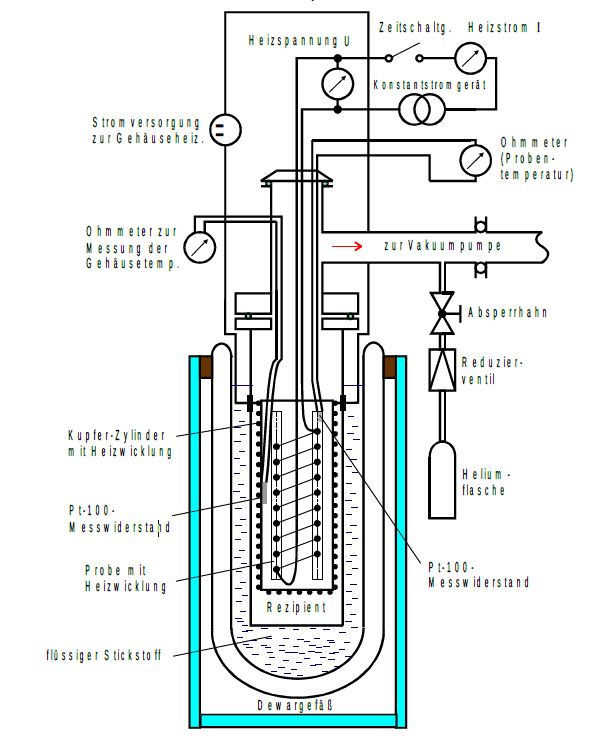
\includegraphics{content/Aufbau.jpg}
  \caption{Schematische Darstellung des Versuchsaufbaus.\cite{manual}}
  \label{fig:aufbau}
\end{figure}


\section{Durchführung}

Zu Beginn des Versuches wird etwaige Luft, die sich in Rezipienten befinden könnte, abgepumpt. Danach wird der Rezipient mit Helium befüllt. Damit wird sichergestellt das sich kein in der Luft enthaltendes Wasser in Rezipienten mehr befindet und der Wärmeaustausch mit dem Wärmebad somit möglichst gleichmäßig stattfinden kann. Das Dewar-Gefäß wird dann mit flüssigem Stickstoff befüllt. Nachdem die Probe auf ungefähr \SI{70}{\K} abgekühlt ist, wird der Rezipient wieder evakuiert, um den Wärmeaustausch der Probe mit seiner Umgebung möglichst gering zu halten.
Zum eigentlichen Messvorgang wird die Probe und der Probenbehälter durch die sie umgebenden Heißwicklungen erhitzt. Die Temperatur wird in gleichmäßigen Abständen von 1:30 Minuten gemessen. Zur Bestimmung der zugefügten Energie wird zudem die Spannung und Stromstärke, die an den Heizwicklungen anliegt aufgenommen. 